%\documentclass{standalone}
%\usepackage{tikz}
%\begin{document}
	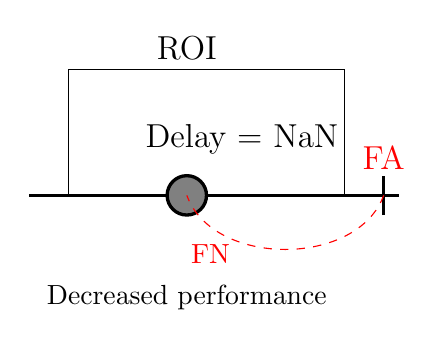
\begin{tikzpicture}[scale=1.0, xscale=1,yscale=1]
		\def\rad{0.25}
		\def\halfh{0.25}
		\draw[black, very thick] (0.5,0) -- (5.2,0);

		% CHP
		\draw[fill=gray, very thick] (2.5, 0) circle (\rad);
		

		% CDE1
        %\node[above] at (2.7, 0.7) {The same as in A};

		% CDE2
		\draw[black, very thick] (5,-\halfh) -- (5, \halfh);
		\node[above, red] at (5, 0.2) {\large FA};

		% ARCH
		\draw[dashed, red] (5,0) to [out=180+70,in=360-70] (2.5,0);
		\node[red] at (2.8,-0.75) {FN};

		% ROI
		\def\hroi{1.6}
		\draw[black] (1,0) -- (1,\hroi) -- (4.5, \hroi) -- (4.5, 0);
		\node[above] at (2.5, \hroi) {\large ROI};
        \node[above] at (3.2, 0.4) {\large Delay = NaN};
		
		\node at (2.5,-1.3) {Decreased performance};
	\end{tikzpicture}
%\end{document}
